\chapter{Konzeption des Frameworks}
\label{chap:konzeption_pubsub}
In diesem Kapitel wird die Konzeption des Frameworks zur Verteilungsoptimierung in seinen Einzelheiten erläutert. Ausgehend von den in \cite{Ficher2010a} identifizierten Eventtypen und Optimierungsdimensionen wird im nächsten Abschnitt beschriebene Problemstellung greifbar. Das Framework muss generisch auf vielfältige Weisen anpassbar sein ohne teure Laufzeiteinbußen zu bedingen \cite{NEW_PAPER} \missing{CITE: NEW PAPER!}. Weiterhin darf die Konzeption, \ac{m2etis} als ein einfach zu nutzendes kanalbasiertes Publish/Subscribe-System zu darzustellen nicht aus dem Fokus geraten. Die Problemstellung führt zum Verarbeitungsmodell das beispielhaft getestet wird.

Im Optimierungsschritt erzeugt \ac{m2etis} für jeden Eventtypen einen optimierten Kanal der über das Publish/Subscribe-System angesprechbar ist. Dieses bieten die bekannten Methoden \emph{subscribe, unsubscribe} und \emph{publish} an. Jeder Kanal ist entlang den Dimensionen derart optimiert, dass Nachrichten des Eventtypen bestmötlich verarbeitet und über Netzwerk verteilt werden können. Das Netzwerk selbst wird über die \ac{kbr}-API angesprochen, die ihrereseits drei Methoden anbietet um den Nutzer über Knotenein- und austritte sowie über den Knoten zu routende und auch ankommende Nachrichten zu informieren \cite{Dabek2003Towards}. Damit ein Kanal nur jene Nachrichten bearbeitet die für ihn bestimmt sind, werden eigene Nachrichtentypen am Netzwerk registriert.

Für die logische Umsetzung der in \cite{Fischer2010Event} identifizierten semantischen Dimensionen eines Eventtypen wird der Begriff \emph{Policy} eingeführt. Eine Policy definiert dabei Schnittstelle für verschiedene konkrete Implementierung (genannt Strategie) und deren Auswirkung auf die Nachrichtenverarbeitung im Publish/Subscribe-System. Die folgenden sieben Policies decken die Dimensionen ab \cite{NEW_PAPER}.\missing{CITE: NEW PAPER!}

\begin{description}
\item[Verteilung] bestimmt die Verteilung der Events und den Aufbau des Multicast-Trees, mittels dem die Nachrichten versandt werden \cite{KostasKatrinis2005}.
\item[Filterung] erlaubt es Anmeldungen Prädikate mitzugeben. Es stellt sicher, dass diese Prädikate nach oben im Multicast-Tree zusammengeführt werden, damit Nachrichten frühzeitig gefiltert werden können. Dies bedeutet, dass Nachrichten jeweils beim logischen Absender gefiltert werden müssen.
\item[Zustellung] bestimmt das Kommunikationspradigma des Nachrichtenversand und leitet z.B. Bestätigungen über eingegangene Nachrichten an den sendenen Knoten ein.
\item[Reihenfolge] definiert die Synchronisationskonzept der Nachrichten in einem Kanal.
\item[Persistenz] bietet die Möglichkeit an verschickte Nachrichten zu speichern.
\item[Sicherheit] gibt eine Schnittestelle zur Nachrichtenverschlüsselung vor.
\item[Validität] prüft die ankommenden Nachrichten auf ihre Validität. Frühzeitig verworfene Nachrichten können das Nachrichtenaufkommen im System stark vermindern.
\end{description}

Die Verbindung der Publish/Subscribe Methoden und der genutzen \ac{kbr} Methoden ist trival, da jede verschickte Nachricht durch die Methoden \emph{forward} und \emph{deliver} des Netzwerkes verarbeitet wird \cite{Dabek2003Towards}.\\
Die Verteilung der Policies auf die verschiedenen Nachrichtentypen ist hingegen interessanter und in \Fref{tab:verbindungsmatrix} aufgezeigt. Bei der Verarbeitung von \emph{Publish}-Nachrichten, den eigentlichen Events, wird jede Policy abgefragt. Die \emph{Subscribe}- und \emph{Unsubscribe}-Nachrichten dienen jedoch nur zum Aufbau und der Verwaltung des Multicast-Treesrm. Aus diesem Grund werden bei diesen Nachrichtentypen nur die Policies Verteilung, Filterung und Sicherheit gebraucht.

Events, also Publish-Nachrichten, werden ausschließlich in deliver behandelt, so dass diese bei allen Empfängern ankommen und unterwegs nicht verändert oder terminiert werden können. Dies ist ein kleiner Schritt in die Richtung zur Betrugsverhinderung. Für Subscribe- und Unsubscribe-Nachrichten entscheided die eingesetzte Verteilungsstrategie darüber, ob diese in forward und/oder deliver behandelt werden. Nur in foward haben die beiden Strategien Verteilung und Filter die Möglichkeit die zu weiterleitende Nachricht zu verändern oder gar zu terminieren. Dies bedeutet, dass jede Filterstrategie generisch beide Varianten unterstützen muss.

\begin{table}[!h]
\resizebox{\textwidth}{!}{%
\begin{tabular}{llccccccc}
\toprule
Nachrichten- & KBR	& \multicolumn{7}{c}{Policy pro Kanal} \\
\cmidrule{3-9}
typ				&	Methode	& Verteilung & Filterung & Zustellung & Reihenfolge & Persistenz & Sicherheit & Validität \\
\midrule
publish	    & deliver & + & + & + & + & + & + & + \\
\midrule
subscribe	  & deliver & + & + &   &   &   & + & \\
\cmidrule{2-9}
			      & forward & + & + &   &   &   & + & \\
\midrule
unsubscribe & deliver & + & + &   &   &   & + & \\
\cmidrule{2-9}
      & forward & + & + &   &   &   & + & \\
\bottomrule
\end{tabular}}
\caption{Verbindungsmatrix}
\label{tab:verbindungsmatrix}
\end{table}


\cite{Fischer2010a, Fischer2010Event}

\cite{BeFiMu2006PubSubQoS}




Typ und Implementierung der einzelen Kanäle verstehen, einfache kanal PubSub-Api anbieten.


\section{Verarbeitungsmodell}

Based on the given mapping, the challenge is to find a generic application order for the policies in the processing model.

For the distribution of a message the routing policy has to provide a list of target nodes, to whom the message must be send. Every multicast-tree has one or more corresponding root nodes. Subscribe or unsubscribe messages are always sent to that nodes, while publish messages from a non-root node must always be sent to the root nodes to trigger the publish process. Such messages are flagged \emph{to root}. On the root nodes, this flag is set to \emph{from root}. Nodes sending messages as \emph{from root} return the list of subscribers as target nodes which are filtered according to their predicate given at subscription. Finally the message is encrypted and handed over to the network.



\begin{figure}[htbp]
\centering
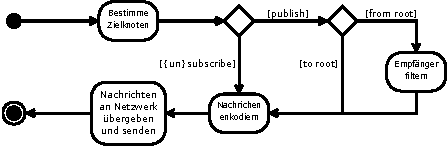
\includegraphics{grafics/processing_send.pdf}
\caption{Verarbeitungsmodell}
\label{fig:processing_send}
\end{figure}

\begin{figure}[htbp]
\centering

\includegraphics{grafics/processing_forward.pdf}
\caption{Verarbeitungsmodell}
\label{fig:processing_forward}
\end{figure}

\begin{figure}[htbp]
\centering
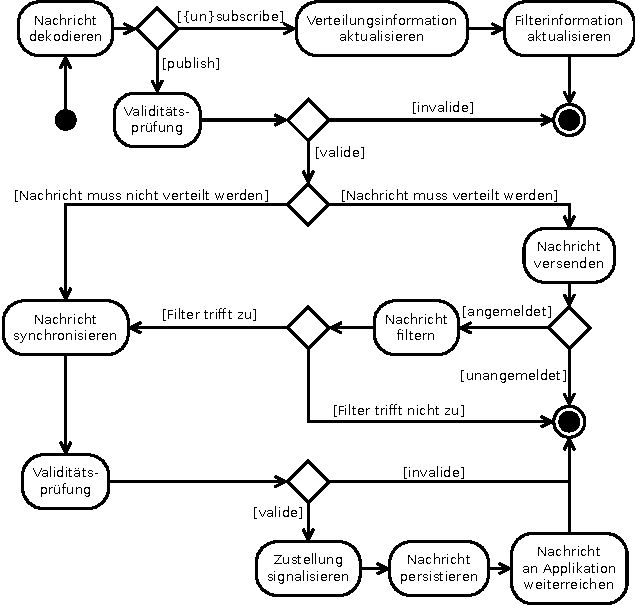
\includegraphics{grafics/processing_deliver.pdf}
\caption{Verarbeitungsmodell}
\label{fig:processing_deliver}
\end{figure}

Decryption is the first action if a message is processed in deliver. After that subscribe and unsubscribe messages are handled separately. These messages are passed to the strategies for routing and filter to alter the multicast tree. Publish messages on the other hand have to pass the validity check. The next step checks whether the message must be spread i.e. distributed to other nodes. That is the case if the actual node is a root node or an intermediate node with distribution responsibility. If yes, the message is distributed using the send-process explained above. Now, the subscription and the predicate of the actual node are checked to ensure a proper delivery if that node is subscribed, too. If the actual node is a simple subscriber and the message is flagged \emph{from root} the predicate is not tested, as it is already checked while sending the message at the publishers side. The two paths merge at the ordering step. As ordering may hold messages back until they are ready the validity has to be checked again. The deliver dimension is called next offering to send acknowledgements back to the sender. Persisting the message is the last action before the message is finally delivered up to the application.\\
The handling in the forward-action from the \ac{kbr} is similar to deliver as the subscribe or unsubscribe information is extracted and passed to the strategies and they may alter the message.

As failures are not detected activeley in such networks, it is important to automatically renew the subscription. If nodes in the logical multicast-tree fail, the messages are automatically routed via other hosts, rebuilding the tree. However, it is possible that some messages are lost during the recovery.

\subsection{Beispielhafte Strategien}
For every policy \ac{m2etis} provides one ore more implementations. For example \emph{Direct} or \emph{Multicast} for routing. The framwork permits inclusion of more user-defined strategies. Different types of channel use a different set of implementations for every policy, creating a variety of optimization options. Each implemented strategy must provide additional cost information that is used in the optimizing step and they may add information onto each message to enable the customized treatment.

Using the example of Scribe \cite{Castro2002Scribe} and VON \cite{Hu2006VON} some details and inner workings of the processing model showed in figure \ref{fig:deliver} are explained. Scribe creates a multicast-tree trying to minimize the amount of messages while an algorithm like VON is neighborhood centric.

Using a scribe-like algorithm for routing \emph{Get Targetnodes} returns either the calculated root node for the channel or the list of subscribed nodes to which a publication must be forwarded. On the other hand a routing strategy like VON returns the in-game neighbors, obtained through application-level knowledge, as each node subscribes at his neighbors in the virtual world. Publications are sent to self enabling the distribution in deliver.

Scribe processes unsubscribe and subscribe messages in forward. Each node on the routing path adds the sender to its list of subscribers and can changes the message to create the multicast-tree. The periodic resubscription is triggerd externally for subscribed nodes as the channel will call its own subscribe method again or internally for intermediate routing hops as the algorithm will resend its subscriptions if other nodes down in the multicast-tree will refresh their subscribtion. It is necessary that the filter strategy is always involved to ensure the correct merge of predicates upwards the logical mulitcast-tree.

VON on the other hand does not need automatic periodic subscriptions, because each node will unsubscribe and subscribe frequently. Using the example of position updates it is obvious that each node and its neighbors move often and need to alter their subscribtions each frame in the game.

Using TTL or a timestamp-based approach for the strategy implementing the validity policy, the TTL would be increased on every routing hop or the passed time since the message was created is tested against the interval set in the strategy.

This exemplary discussion of different strategies indicates the generic nature of our processing model in terms of a multidimensional optimization for publish/subscribe channels.
